\documentclass[]{article}
\usepackage{graphicx}
\usepackage{amsmath,amsfonts,amssymb}
\usepackage[font=small,labelfont=bf]{caption} % Required for specifying captions to tables and figures
\graphicspath{ {./Images/} }

%opening
\title{Computer Vision Assignment Two @ ETH Zurich \\ \large Feature Extraction}
\author{Ossama Ahmed 18-936-872}

\begin{document}

\maketitle

\section{Introduction}\

Feature extraction is used in many application in Computer Vision such as motion detection, vistual object tracking, image reconstruction..etc. 

In this assignment we implement the harris corner detector and then we perform feature matching. The results obtained are then compared to the SIFT detector.
\newline

\section{Feature Extraction}\



First we compute the gradients in  x and y direction using the built-in function in matlab that takes care implicitly for the boundary cases in the image. Afterwards, the image is smoothed using a gaussian filter and the components needed for the harris corner detector are calculated which are then used to calculate the response measure. Through plotting the  histogram of the response measure of all the image pixels; an initial estimate of the threshold is observed.


\medspace
$\
H =
\begin{bmatrix}
I_x^2       & I_x*I_y \\
I_x*I_y      & I_y^2\\
\end{bmatrix}$
\newline
\medspace



$\
K = det(H) / trace(H) = (I_x^2 * I_y^2 - (I_x * I_y)^2) / (I_x^2 + I_y^2 + eps)$

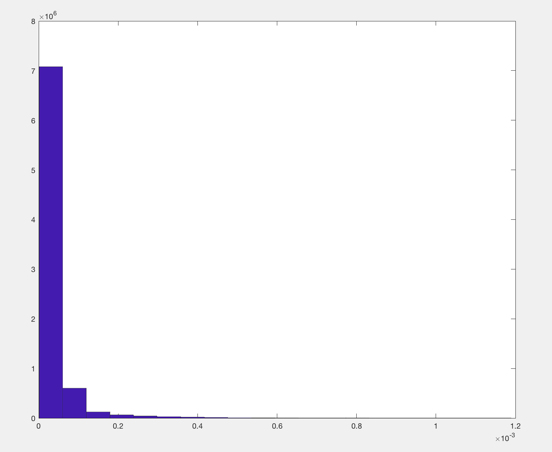
\includegraphics{histogram.png}
\captionof{figure}{Harris Corner Response}

Afterwards, non max supression is applied to the K global matrix without removing the response measures that are below the threshold (for faster performance). To apply the non max supression on the whole matrix, ordfilt2 was used and a 3x3 window. 

To determine the final keypoint features. A boolean expression is used. 
$\ KeyPoints = (nonmax == K)  \&   K > threshold$

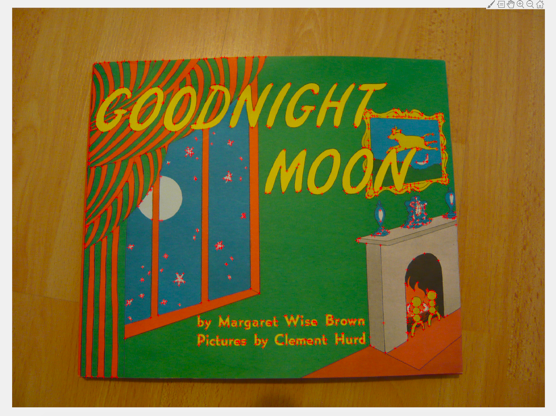
\includegraphics{l1_corners.png}
\captionof{figure}{Corners using Harris Detector in Image 1}

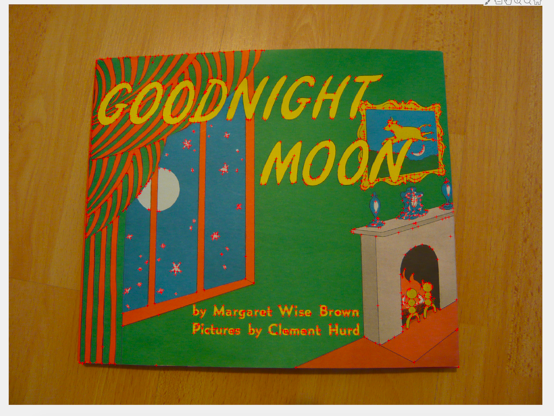
\includegraphics{l2_corners.png}
\captionof{figure}{Corners using Harris Detector in Image 2}

Number of corners in Image 1 = 886 \newline
Number of corners in Image 2 = 1122

\section{Feature Descriptor}\

For each key point, we save the patch around it as a decriptor in a 3x3 window, so we can compare the two descriptors available from the two images to deduce the matches.

\section{SSD Feature Matching}\

For each key point descriptor in one image, we detect if there is a corresponding key point in the other image where the squared difference is really small that we can be confident that it's an actual match of the point. The threshold used to define how small the square difference should be so that it can be accepted as a match, was caclulated using trial and error. Small differences denote high similarity.

Total Number of Matches =  224

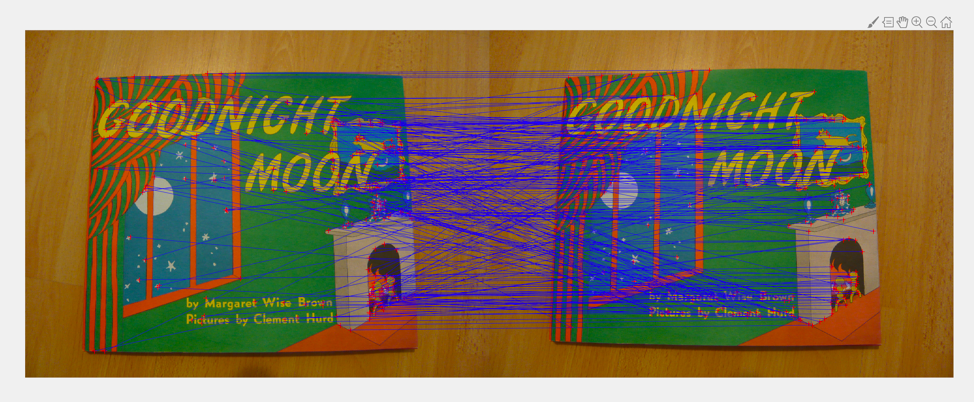
\includegraphics{harris_matching.png}
\captionof{figure}{Feature Matching using the Harris Corner Detection Results.}

\section{SIFT Features using VLfeat}\

The tutorial to use VLFeat (SIFT feature extractor from Andrea Vedaldi) was followed to apply SIFT on the two images provided. The features were extracted using SIFT detector and then matched.
To decrease the number of non sharp corners detected by the default values of the toolbox, a peakthreshoild was used and set to 8. Below are the results obtained from the tool box. \newline

Total Number of matches = 365


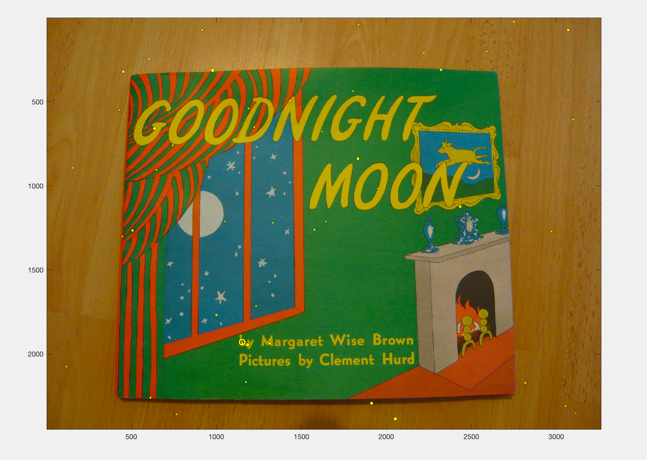
\includegraphics{tool1.png}
\captionof{figure}{ToolBox Result 1}

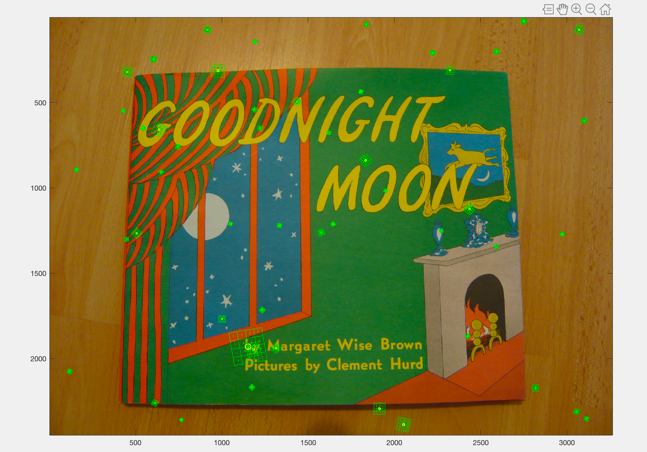
\includegraphics{tool2.png}
\captionof{figure}{ToolBox Result 2}


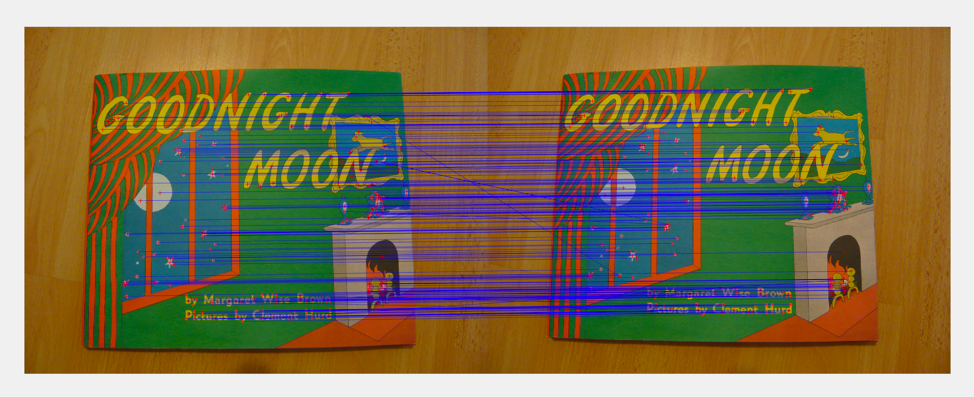
\includegraphics{tool3.png}
\captionof{figure}{ToolBox Result 3}

\section{Conclusion}\

It's obvious from the results above that the SIFT feature extractor produced more accurate results than the Harris corner detector; which was expected. Also, the keypoints detected with SIFT are less noisy. The harris detector can do a better job than the above image with tweaking both thresholds (the key points threshold and the matching SSD threshold). Tweaking the thesholds was a manual effort, I am sure if I experimented with more values or an automatic tuning way; I will obtain better results for the Harris detector compared to the above results.

\end{document}
